\chapter{Symbolic Security Analysis Using Scyther}
\label{chp:scyther} 

%Introduction to Scyther. What it is. How it works. Examples.

There exist multiple state-of-the-art tools for performing formal analysis of security protocols, for example Avispa \cite{avispa}, ProVerif \cite{proverif}, Tamarin Prover \cite{meier2013tamarin}, and Scyther \cite{scyther}. This thesis uses Scyther as its tool for conducting formal security analysis. It is chosen on suggestions from C. Boyd and B. Hale, and also on a review of popular formal security analysis tools in \cite{tool-compare}. Another reason for choosing Scyther is its relatively easy syntax that resembled syntax from well-known programming languages. Tamarin was also considered, but it requires that protocols are modelled using multiset rewriting and first-order expressions \cite{multiset, meier2013tamarin}. The following chapter will give an introduction to Scyther, how it works, and examples of usages.




\section{The Scyther Tool: Verification, Falsification, and Analysis of Security Protocols}

Scyther is a tool for verification, falsification, and analysis of security protocols developed by Cas Cremers. The tool is based on a pattern refinement algorithm that enables unbounded verification, falsification, and characterization \cite{cremers2008scyther}. Scyther allows its users to verify security protocols in two different ways. The first option is to execute Scyther scripts through the command-line interface, which provides an output file containing the results of the protocol verification. Option two is to use Scyther's own \gls{gui}, which provides panels for both verification results, and in case of attacks being found, a visual graph of Scyther's proposed attack on the protocol. The most recent release of Scyther was published on April 4, 2014, and is currently available for Windows, OS X, and Linux.

% Ok

Security protocol specifications are built up of messages that are sent between different entities and computation that is done at either side. Much like a blueprint, these specifications define what a protocol is allowed to do, and how it is allowed to communicate \cite{cremers2003defining}. The blueprint can be modelled by Scyther, where the entities are converted into roles, the messages are converted into send and receive events, and the security requirements into claim events. These terms are explained in the sections to follow. Scyther performs complete characterization of a protocol, where roles are broken down into a finite set of representative behaviours by analysing all the possible execution traces where the events hold. The intuitive idea behind this algorithm is that the set of execution traces together represents all possible ways in which the protocol can execute. These traces are then grouped into patterns, which are partially ordered, symbolic sets of events \cite{cremers2006scyther}. From the patterns, Scyther is able to construct a complete set of attack traces for each security claim. When analysing protocols, the realizable traces are compared to the attack traces. If none of these realizable traces of the protocol exhibits an attack trace, then no attack exists, and the security property is verified. 

Most protocols can be characterized into a finite set of traces, which enables Scyther to perform \emph{unbounded} verification of the protocol. This greatly differs from the majority of other verification tools which perform \emph{bounded} verification \cite{cremers2008scyther, cremers2009comparing}. When performing bounded verification, there exists a finite set of traces that the tool is able to verify, meaning that the entire space of possible states is not covered in the verification process \cite{cremers2008unbounded}. At best, such a verification can guarantee that the security requirements hold under a finite subset of the actual state-space. Unbounded verification, however, is to verify all possible states, or behaviours, of the protocol which is a great enhancement compared to bounded verification algorithms. In addition to handling an infinite state-space, Scyther is also guaranteed to terminate, which gives it the ability to provide useful results even when it is not able to establish unbounded correctness, or in the scenario of where no attack is found.

As mentioned, a protocol specification contains a set of roles which serves as a blueprint that describes what the protocol is allowed to do. When executing the protocol, each of the different roles can be executed multiple times, and in parallel with each other by one or more agents \cite{cremers2006scyther}. The execution of a role is referred to as a \emph{run}, and defines a unique instance of the protocol with respect to local constraints and the binding between the role and the actual agent acting out the role's behaviour. Scyther allows its users to state security claims which are evaluated as they appear in the protocol trace, either ending in a successful verification of the security property or in a failure. In the presence of a failure, Scyther will provide a concrete attack on the protocol by utilizing one of the attack traces from the pattern, and it will also present an attack graph to illustrate the threat. If the protocol developer is unsure of what types of claims should be stated for each role, Scyther has support for so-called verification of automatic claims, where Scyther will provide general claims such as secrecy for keys and values, and authentication of communicating parties.

Another of the major novelties in Scyther is the possibility for performing so-called multi-protocol analysis, which essentially means analysing multiple protocols that co-exist in the environment. Such an analysis has previously been infeasible because of an incredibly wide state-space, but thanks to Scyther's unique algorithm that operates on an unbounded state-space, it allows for multi-protocol analysis.

Scyther is available in two versions. The first version is a plain implementation of Scyther, while the second version also contains options for creating a stronger adversary compromise model than the Dolev-Yao model. The compromise edition contains different \gls{lkr} rules, which are used for modelling different adversary capabilities such as \gls{kci}, \gls{wpfs}, and \gls{pfs}, along with support for known-key security. 


\section{Scyther Syntax}


The syntax used in \gls{spdl} files, which are protocol files that can be run and verified by Scyther, can resemble popular object-oriented languages such as C, C++, or Java. Listing \ref{lst:example} contains the structure of a minimum working example of a protocol we call Test, consisting of an outer class defining the protocol and multiple agents (or roles) inside the protocol. In this example, we define that our protocol consists of two communicating parties, U and V, without any specific behaviour.\newline

\begin{lstlisting}[caption={Example of the structure of a protocol modelled in Scyther, consisting of roles with different behaviours.}, label={lst:example}, style=code-listings]
protocol Test(U, V){
	role U { };
	role V { };  
};
\end{lstlisting}

For each of the different roles in the protocol, behaviour can be added as a sequence of send and receive events, as well as variable declarations, constants, and claims. For the role U, we can define a simple behaviour as shown in Listing \ref{lst:roleu}, where U generates a random nonce \texttt{Ru} and sends it to V, before receiving a message from V containing the random nonces \texttt{Ru} and \texttt{Rv}. All events are labelled with either \texttt{send} or \texttt{recv} followed by a subscript and a number. The number indicates the message's position in a \gls{msc}, and must be incremented for each message sent.\newline

\newpage

\begin{lstlisting}[caption={Terms can be generated, sent, and received when communicating with other agents.}, label={lst:roleu}, style=code-listings]
role U{
	fresh Ru: Nonce; # Freshly generated nonce
	var Rv: Nonce; # Variable for receiving a nonce
	
	send_1(U, V, Ru); # Send message to V containing Ru
	recv_2(V, U, Ru, Rv); # Receive message from V containing Ru and Rv. The received Rv value is stored as the variable Rv.
};
\end{lstlisting}



Typically, a \texttt{send}-event has a corresponding \texttt{recv}-event at the receiving role with the same number.\newline


\begin{lstlisting}[caption={Events in Role V usually corresponds to events in role U.}, style=code-listings]
role V{
	[...]
	
	recv_1(U, V, Ru); # Receive message sent from U containing Ru. The received Ru nonce is stored as the variable Ru. 
	send_2(V, U, Ru, Rv); # Send message to U containing the received nonce Ru and the freshly generated Rv. 
};
\end{lstlisting}


Along with support for creating fresh nonces, variables, and terms, Scyther also provides a wide set of cryptographic elements such as hash functions, symmetric-key cryptography, and public-key cryptography. Scyther also allows for declaring user specific types and macros, which are abbreviations of complex expressions. In Listing \ref{lst:crypt}, a hash function is used to define a function that generates a \gls{mic} (which is essentially the same as a \gls{mac-auth}). On the next line, we have created a macro representing the generation of a pairwise key between U and V. The key is represented as an encryption of the two values \texttt{Ru} and \texttt{Rv} using a symmetric key that is shared between U and V. Constants and functions defined outside of a role are considered to be global, and available to all of the defined roles in the protocol. When the protocol run reaches the \texttt{send\_3} event, it looks up the macro for pairwise key and computes it by encrypting the \texttt{Ru} and \texttt{Rv} values using the symmetric key shared between U and V. \texttt{send\_3} also contains an example of a \gls{mic} of the constant \texttt{msg} sent from U to V, which is created by hashing the message and the pairwise key together using the predefined hashfunction \texttt{MIC}.\newline


\begin{lstlisting}[caption={Example of how to use hashfunctions, macros and encryption.}, label={lst:crypt}, style=code-listings]
hashfunction MIC; # An hashfunction to represent a Message Integrity Code (MIC) generation.

macro PairwiseKey = {Ru, Rv}k(U, V);

role U {
	[...]
	const msg;
	send_3(U, V, {msg}PairwiseKey, MIC(msg, PairwiseKey)
}
\end{lstlisting}


\subsection{Security Claims}
\label{subsec:claims}

A sequence of events within a role is usually followed by a set of claim events. Claim events are used for describing security properties of a role, for example that some value should be considered secret, or that certain properties hold for authentication. Such claims can be formally verified by Scyther. If the protocol is not instructed with any security claims, Scyther is able to generate general claims for claiming secrecy for keys and values that are sent between roles, as well as authentication for communicating parties, by using the ``Verify automatic claims'' alternative provided by the \gls{gui}.

\subsubsection{Secret}


The first, most trivial security claim is secrecy. Secrecy expresses that the stated property is to be kept hidden from an adversary, even in the case of where the adversary controls the network used for communication. However, if one of the agents gets compromised by the adversary and the protocol is executed between an honest agent and the adversary, it would in the end learn what was meant to be kept hidden from it \cite{cremers2005operational}. The secrecy claim does not hold for such cases (nor is it intended to), but for each case where the protocol is executed between two honest agents where the secret property is successfully kept hidden from the adversary. For our example protocol, we can claim that the two values \texttt{Ru} and \texttt{Rv} are supposed to be secret and thereby hidden from the adversary as shown in Listing \ref{lst:cl-sec}. These claims will obviously fail as we have not specified that any encryption should be used on the messages that are passed between the two roles.\newline

\newpage

\begin{lstlisting}[caption={Example of how to claim secrecy for terms in Scyther.}, label={lst:cl-sec}, style=code-listings]
role U{
	[...]
	
	# Claims:
	claim_F1(U, Secret, Ru);
	claim_F2(U, Secret, Rv);
};
\end{lstlisting}




\subsubsection{\gls{skr}}

Session keys are created at the end of a key establishment process, and are usually used for a session of the communication, before being replaced. When they expire, they are deleted from the system and never used again, limiting the amount of ciphertexts available for the adversary to perform cryptanalysis. In Scyther, the claim \gls{skr} is used to identify the session keys in the protocol, and claim that they are secret. \gls{skr} can be used by Scyther to model unknown key share attacks (as described in Section \ref{sec:attributes}), where Scyther will reveal any session key to the adversary, given that its session identifier (i.e. run identifier) differs from the current session's \cite{cremers2014improving}. In order to use Scyther's \gls{skr} claims, the compromise edition has to be used, and the session-key reveal checkbox needs to be checked in the settings. If the \gls{skr} claim is used without enabling this setting, the claim is verified as a regular secrecy claim as defined above.

%\gls{skr} is mostly the same as the regular secrecy claim, but is used to highlight that the term that is claimed to be secret is also a session key. This instructs Scyther to reveal the session key to the adversary after it has executed its run, hence proving that the session keys are working correctly, and that current session keys are kept secret from the adversary \cite{scyther-manual}.  If not, this claim is identical to the ordinary secrecy claim presented above.



\subsubsection{Aliveness}

Aliveness is considered to be the weakest form of authentication, guaranteeing to the party stating the claim (U) that if the protocol is completed successfully, then the communicating party (V) has previously executed the protocol \cite{lowe1997hierarchy}. This does not necessarily mean that U knew he was interacting with V, nor does it mean that V has executed the protocol any time recently.


\subsubsection{Weak Agreement}

Weak agreement strengthens the authentication form introduced as aliveness. Such an authentication states that the responder in fact was executing the protocol with the initiator (U), and not just having run the protocol at some point \cite{lowe1997hierarchy}. By claiming that the protocol holds under the weak agreement, we state that if U successfully completes a run with the intended responder (V), then V also believes that it has previously run the protocol with U. Such a claim would prevent an adversary from acting as a responder by running another run of the protocol in parallel with a run with U, and conducting a man-in-the-middle-attack. The Needham-Schroeder case presented in Chapter \ref{chp:background} failed on this claim, allowing Lowe to construct his attack. 


\subsubsection{Non-injective Agreement}

Where the authentication provided by weak agreement does not specify which of the two communicating parties acted as initiator and responder, non-injective agreement does. It guarantees that if the initiator (U) successfully completes a run of the protocol, apparently with the responder (V), then V has completed a run with U, where he acted as a responder \cite{lowe1997hierarchy}. This does, however, not indicate that they both have executed exactly one run. There is still a possibility that U has executed multiple runs with a responder which he believed to be V, but may in fact have been communicating with the adversary. Another guarantee provided by non-injective agreement is that if U also sends a set of variables to V in the completed run, then they both agree that the exchanged data values correspond to all of those in the set of variables. In Listing \ref{lst:cl-auth}, the example protocol claims that V is ``alive'', has run the protocol at some time with U, and that during this particular run, it was U and V that were communicating.\newline

\begin{lstlisting}[caption={Example of how to claim authentication by use of alive, weak-agreement, and non-injective agreement.}, label={lst:cl-auth}, style=code-listings]
role U{
	[...]
	
	# Claims:
	claim_U1(U, Alive);
	claim_U2(U, Weakagree);
	claim_U3(U, Niagree);
};
\end{lstlisting} 


\subsubsection{Non-injective Synchronization}

Synchronization requires that all protocol messages occur in the expected order with their expected values, and that the behaviour is equivalent to as if the protocol was executed without the presence of any adversary \cite{cremers2006injective}. The \emph{injective synchronization} property states that the protocol executes as expected over \emph{multiple} runs, claiming that it is not possible for an attacker to use information from previous runs to disrupt the current protocol execution \cite{cremers2005operational}. Such an attack is known as a replay attack, and is used by an adversary to inject traffic into the protocol execution to induce undesirable or unexpected behaviour. Scyther, however, does not support this enhanced form of synchronization, hence it strongest type of synchronization is \emph{non-injective synchronization}. Because of this, Scyther is not able to verify whether or not a protocol is secure against replay attacks. Listing \ref{lst:cl-synch} contains an example on how to claim non-injective synchronization for the example protocol.\newline

\begin{lstlisting}[caption={Claim for declaring non-injective synchronization in Scyther.}, label={lst:cl-synch}, style=code-listings]
role U {
	[...]

	# Claims:	
	[...]
	
	claim_U4(U, Nisynch);
}


\end{lstlisting}

%Synchronization = Strong form for authentication. Does not protect against replay attacks. Same for Non-injective synchronization.


\subsubsection{Running, Commit}

Running and commit signals can be used as a form of authentication over variables that are sent in a message. By using these signals (in Scyther modelled as claims), we can verify that a variable sent from U to V, and then returned to U, has not been changed from its initial value during transmission. From a formal view, this can be seen as non-injective agreement over a set of terms \cite{scyther-manual}.

The expression $claim(V, Running, U, Ru)$ denotes that V is currently executing the protocol with U, and with the nonce $Ru$. In U's case, $claim(U, Commit, V, Ru)$ indicates that the protocol as reached a point where authentication is claimed (U has completed the protocol run with V), where $Ru$ is the variable that is claimed to be exchanged during this part of the run \cite{ryan2001modelling}. Usually, the \emph{commit} claim is stated at the end of the protocol run. For the correctness of the \emph{commit} claim to hold, it requires that the \emph{running} signal is added in the communicating role, and preceding the \emph{commit} claim in the trace.

This pattern is a scheme for authentication properties, but it also allows for expressing authentication for additional information specific to a certain part of the protocol run, for example some variable inside the message. Occurrence of a \emph{commit} signal in U's protocol run means that a corresponding \emph{running} signal has previously occurred in V's protocol run, which guarantees that the received message containing $Ru$ must have been transmitted by V \cite{ryan2001modelling}. Listing \ref{lst:cl-rc} contains an example of how we can claim non-injective agreement over a variable, in this case the nonce $Ru$. 
\newline
\newpage
\begin{lstlisting}[caption={Example of running and commit claims in Scyther to provide authentication for a set of terms.}, label={lst:cl-rc}, style=code-listings]
role U{
	[...]
	
	send_1(U, V, Ru);
	recv_2(V, U, Ru, Rv);
	claim_U5(U, Commit, V, Ru); # Authentication over the term Ru is claimed
};

role V{
	[...]
	
	recv_1(U, V, Ru);
	claim_V6(V, Running, U, Ru); # Claim that V is currently running the protocol with U with the value Ru
	send_2(V, U, Ru, Rv); 
}
\end{lstlisting}

\section{Defining an Adversary Compromise Model}
\label{sec:adversary}

% https://www.inf.ethz.ch/personal/basin/pubs/esorics10.pdf

Formal adversary models are described in Section \ref{sec:formal}. Compromise of long-term keys can, for example, allow an adversary to recover previous session keys (and future) and decrypt the traffic if the protocol does not provide forward secrecy. Another option is for the adversary to perform \gls{kci} where it impersonates the victim towards other agents, or impersonate other entities in communication with the victim. Scyther allows for customizing different adversary models through its settings for an adversary compromise model, which enables a strong Dolev-Yao style adversary with support for verifying security properties such as \gls{pfs}, \gls{wpfs}, \gls{kci} and known-key security. These security properties are decomposed in Table \ref{tab:sec-prop-adv-mod} into their basic property, type of security property, and what adversary model (which will be elaborated in the next section) provides them.

\begin{table}[h]
\centering
\begin{tabular}{|l|l|l|}
\hline
Security property                   & Basic property           & Adversary model    			\\ \hline
\gls{kci} 							 & Authentication           & \{\gls{lkr}, Actor\}        	\\ \hline
\gls{pfs}      						 & Secrecy                  & \{\gls{lkr}, After\}        \\ \hline
\gls{wpfs} 						     & Secrecy                  & \{\gls{lkr}, Aftercorrect\} \\ \hline
Known-Key Security                  & Session key secrecy 		 & \{SKR\}                		\\ \hline
\end{tabular}
\caption[Relationship between security properties and the adversary models in Scyther.]{Relationship between security properties and the adversary models in Scyther \cite{basin2010modeling}.}
\label{tab:sec-prop-adv-mod}
\end{table}

\newpage
%\subsection{Compromising of long-term keys}

The initial adversary in the Dolev-Yao intruder model has access to the long-term keys of the communicating parties that do not participate in the current run of the protocol. In other words, if $A$ and $B$ are communicating with each other, then the adversary has access to $C$'s private long-term key during the execution of the protocol. Scyther's initial intruder model, however, does not have access to these keys without directly specifying it in its \gls{lkr} settings \cite{basin2010modeling}.
%When enabling \{\gls{lkr}, Others\}, the adversary is identical to the Dolev-Yao intruder model, and has access to the long-term private keys for other agents than the those currently involved in the protocol execution

Section \ref{sec:attributes} mentioned \gls{kci}, where an adversary in possession of $A$'s long-term private key is able to impersonate $A$ when communicating other agents, or impersonate other entities when communicating with $A$. Such an attack can be modelled by enabling \{\gls{lkr}, Actor\} in Scyther's adversary compromise model. Forward secrecy is the security property where previous communication is protected in the case of compromise of the long-term key, and is enabled in the adversary model by specifying \{\gls{lkr}, Aftercorrect\} or \{\gls{lkr}, After\}. These properties restricts the compromise of long-term keys to only occur after the protocol execution \cite{basin2010modeling}. \{\gls{lkr}, Aftercorrect\} is used to model \gls{wpfs}, and is the weaker case of forward secrecy, where the adversary is considered to be \emph{passive}. For the adversary model, this would restrict it from both injecting messages and obtaining the private keys of the communicating parties after the protocol run.  \{\gls{lkr}, After\} models an \emph{active} adversary capable of actively interfering with the protocol during it run while obtaining the long-term private keys, hence protocols able to provide secrecy in the present this adversary is said to provide \gls{pfs}. 



Figure \ref{fig:compromise-model} illustrates the different \gls{lkr} rules in two dimensions; \emph{when} a compromise occurs, and \emph{whose} long-term keys are compromised. The rows indicate when the compromise occurs, and can either be before the run, during, or after. Columns describe whose keys are compromised, where actors are agents that execute the protocol, peers are communicating partners during the execution, and others are agents not participating in the protocol run. The different capabilities are captured and labelled as different \gls{lkr} rules, as shown on the right hand side of the figure. 

\begin{figure}
	\centering
	\includegraphics[scale=0.60]{compromise-model.png}
	\caption[Figure of the mapping of Long-term Key Reveal rules.]{Mapping of LKR rules. Rows display when the compromise occurs, columns display whose data gets compromised, and the boxes captures the capabilities of the different adversaries, which are labelled to the right \cite{basin2010modeling}.}
	\label{fig:compromise-model}
\end{figure}


In addition to compromising long-term keys, Scyther is also able to model the security property known-key security. By enabling the \gls{skr} rule, the adversary is allowed to obtain all session keys whose session identifier (the identifier of that particular run of the protocol) differs from the current run's identifier.


\section{Scyther's Graphical User Interface}

As mentioned, Scyther provides a \gls{gui} for quickly understand and assess the security of a protocol. If we continue our example of the protocol Test from the section on Scyther's syntax, we now want to verify all the stated security claims. By using the \gls{gui}, we can configure the verification process by stating a maximum number of runs, the adversary compromise model, as well as more advanced options for how to prune the search space. Scyther provides three options in its \gls{gui}: verification of claims, verification of automatic claims, and characterization of the protocol \cite{cremers2008scyther}. Figure \ref{fig:scyther-verify-claims} contains the results of running a verification of the claims previously described for a secure protocol.

\begin{figure}[h]
	\centering
	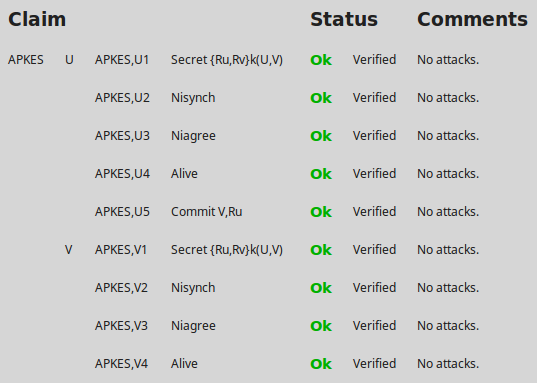
\includegraphics[scale=0.8]{ScytherVerifyClaims.png}
	\caption{Results of a verification process using Scyther where all claims are successfully verified.}
	\label{fig:scyther-verify-claims}
\end{figure}

When no attacks are found, Scyther provides one of two comments: \emph{No attacks within bounds} or \emph{No attacks}. In the first case, Scyther was not able to find any attacks within the bounded state-space, meaning that it may or may not be an attack in the unbounded state-space. The latter, however, states that there was not found any attacks within both the bounded and the unbounded state-space. In this case, Scyther can construct a formal proof of the absence of any attacks, hence the security property is successfully verified. Scyther returns an \texttt{Ok} status code and a \emph{Verified} message for each claim that is successfully verified. As we see in Figure \ref{fig:scyther-verify-claims}, Scyther is not able to find any attacks on the protocol. To illustrate the case of Scyther actually finding an attack, we try to verify the claims introduced in the paragraph on secrecy in Section \ref{subsec:claims}, claiming that \texttt{Ru} and \texttt{Rv} are secret. In our example protocol, both nonces are sent in plaintext between U and V, hence this claim will naturally fail, as seen in Figure \ref{fig:scyther-verify-claims-fail}.


\begin{figure}[h]
	\centering
	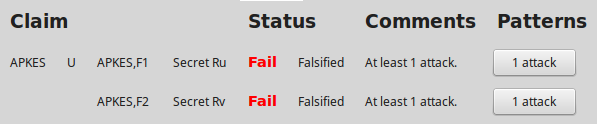
\includegraphics[scale=0.84]{ScytherFailSecretClaim.png}
	\caption{Results of a verification process using Scyther when a claim fails.}
	\label{fig:scyther-verify-claims-fail}
\end{figure}

The status \emph{Falsified} states that the claim is provable false. When a claim is proved to be false, Scyther will also provide a comment; either \emph{At least X attack(s)} or \emph{Exactly X attack(s)}. In the first case, X attacks where found by Scyther, but the search is not able to detect whether or not there may be other attacks as well. In the other case, Scyther can prove that within the given state-space, there are exactly X attacks.

Whenever Scyther finds an attack on a protocol, it will also provide a concrete illustration of the attack as a graph. Figure \ref{fig:scyther-graph} shows an example of such a graph. The top box for each vertical alignment of boxes describes the run, which is confined inside the grey boxes. It contains a description with the identifier of the run, instance type (i.e. what type of role it is running as), which agents it assumes it is communicating with, and also what fresh values that are generated and instantiated in the run \cite{scyther-manual}. Boxes symbolises events in the different runs, connected by arrows which symbolises ordered constraints. Incoming arrows do not indicate that the messages is sent directly in this step, but is merely an ordering stating that this message can only be received \emph{after} something else has happened. For example, in Figure \ref{fig:scyther-graph}, the \texttt{recv\_2} event in \texttt{Run 1} can only happen after Bob has sent his message in the \texttt{send\_1} event and Alice has sent her message in the \texttt{send\_2} event.



\begin{figure}[h]
	\centering
	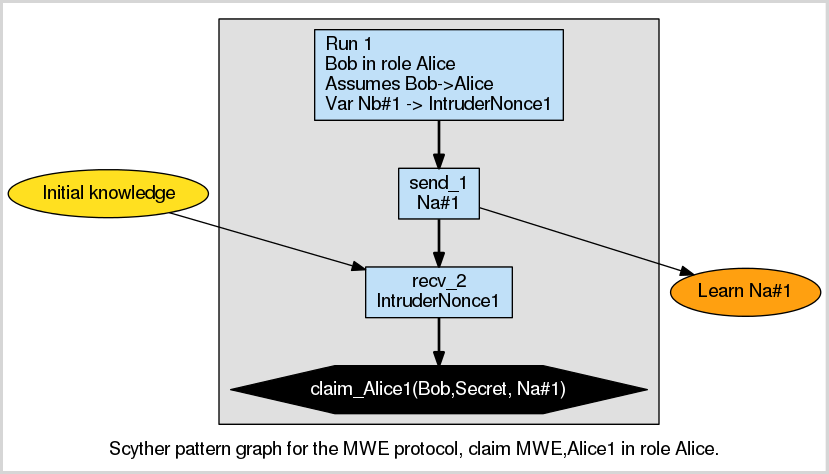
\includegraphics[scale=0.5]{ScytherFailAttackGraph.png}
	\caption{When Scyther finds an attack on a protocol, if will also provide a graph of the attack.}
	\label{fig:scyther-graph}
\end{figure}

Arrows in Scyther graphs can be coloured differently. Red arrows indicate that the sent message does not correspond to the received message, which means that the adversary used some information from the sent message in order to construct the one that is received \cite{scyther-manual}. Green arrows indicates that the sent message is identical to the received message. The last possible color (other than black, which does not carry any specific information) is yellow. Yellow arrows indicate that the two parties agree upon the message that is exchanged between the two, but do not agree upon who was the sender and receiver during the exchange.

When a message is sent, it is instantly obtained by the adversary. Initial knowledge (or intruder knowledge) corresponds to the intuition that the intruder is able to generate fresh values of any type, which it in Figure \ref{fig:scyther-graph} uses to generate the nonce that is sent in the \texttt{send\_2} event. The green oval shape indicates where the adversary obtains the information which falsifies the claim, which in this example is the \texttt{Ru} value that is sent in plaintext. The two last boxes in the graph are the black box at the bottom of \texttt{Run 1} which contains the claim that is falsified by Scyther, and the white box to its right which contains abbreviations of the messages that are passed between roles to increase the readability of the graph.


% More. What do we see?
